%%%%%%%%%%%%%%%%%%%%%%%%%%%%%%%%%%%%%%%%%%%%%%%%%%%%%%%%%%%%%%%%%
%%%  ISWC 2015 Poster: DOREMUS: Doing Reusable Musical Data  %%%%
%%%%%%%%%%%%%%%%%%%%%%%%%%%%%%%%%%%%%%%%%%%%%%%%%%%%%%%%%%%%%%%%%

\documentclass{llncs}
\usepackage{graphicx}
\usepackage{amsmath}
\usepackage{todonotes}
\usepackage{hyperref}
\usepackage{amssymb, bm}
\usepackage{indentfirst}
\usepackage{url}

%%%%%%%%%%%%%%%%%%%%%%%%%%%%%%%
%%%  Beginning of document  %%%
%%%%%%%%%%%%%%%%%%%%%%%%%%%%%%%

\begin{document}

\title{DOREMUS: Doing Reusable Musical Data}
%alternative title: Dataset recommendation for data interlinking - a topic-based approach

\author{Manel Achichi$^1$, Rodolphe Bailly$^2$, C\'{e}cile Cecconi$^2$, Marie Destandau$^2$, Konstantin Todorov$^1$, Rapha\"{e}l Troncy$^3$}
\authorrunning{Achichi \textit{et al.}}
\institute{$^1$University of Montpellier, $^2$Philharmonie de Paris, $^3$Eurecom}% \\ \textit\{\}@lirmm.fr \\ }

\maketitle

%%%%%%%%%%%%%%%%%%
%%%  Abstract  %%%
%%%%%%%%%%%%%%%%%%

\begin{abstract}
This paper introduces DOREMUS---a semantic web project aiming to provide common knowledge models and shared multilingual vocabularies to cultural institutions, publishers, distributors and users in the musical domain. The project develops methods to describe, publish, connect and contextualize music catalogs on the web of data. Our focus is on the description of classical and traditional musical works as well as their interpretations (events).
\end{abstract}

%%%%%%%%%%%%%%%%%%%%%%%%%
%%%  1. Introduction  %%%
%%%%%%%%%%%%%%%%%%%%%%%%%

\section{Introduction}
\label{sec:introduction}
Music is everywhere---played,  recorded, broadcasted and listened to. Files of recorded music are all over the web---stored, streamed, shared or sold. The knowledge about musical works is described in detail in the information systems of several cultural and media organizations around the world. The leading actors in France---the  BnF (\textit{Biblioth\`eque Nationale de France}), the \textit{Philharmonie de Paris} and \textit{Radio France}, as well as the \textit{Meaning Engines} company join forces with three academic institutions within the DOREMUS project\footnote{\url{http://www.doremus.org}} in order to make this knowledge available and re-usable on the web of data. The project covers three main objectives: (1) to publish and to link musical data on the web of data including the description of musical works as well as their interpretation (event); (2) to develop tools assisting the selection of pieces of music, for instance, to generate an original playlist for a specialized radio station or to illustrate a musical period or genre; and (3) to construct and validate educational tools that enable the deployment of standards, vocabularies and the underlying semantic web technologies in the cultural institutions in France and worldwide.

In this paper, we describe our approach for publishing and interlinking descriptions of musical data based on ontological models and vocabularies and we discuss several applications. The goal is to exploit as much as possible the rich data which is available and to open it to the public. The main contributions consist in (1) the provision of advanced ontological models for describing musical works and events and (2) the generation of automatic methods for opening musical data that are initially given in a specific input format, so far, disconnected from the semantic web world.

%%%%%%%%%%%%%%%%%%%%%%%%%%%%%%%%%%
%%%  2. Modeling Musical Data  %%%
%%%%%%%%%%%%%%%%%%%%%%%%%%%%%%%%%%

\section{Modeling Musical Data}
\label{sec:modeling}
Musical works are complex objects. Expressing them comprehensively requires the description of their physical manifestations (recordings, scores) and all the events that define them (creation, publication, performance). The first aspect is relatively well-mastered, in library catalogues as well as in the music industry. Several models can be used to describe a musical work, some being specific to the music domain (MusicOntology), while others being more broadly designed for libraries in general (FRBR\footnote{\url{http://www.ifla.org/publications/functional-requirements-for-bibliographic-records}}, UNIMARC\footnote{\url{http://www.ifla.org/publications/unimarc-formats-and-related-documentation}}). The second aspect is rather new, although there is a growing need and interest in using even-based models. Several ontologies aim specifically to define events (Event\footnote{\url{http://purl.org/NET/c4dm/event.owl}}, LODE\footnote{\url{http://linkedevents.org/ontology/}}), but there are fewer examples of using them to describe the creation and publication processes.
\begin{figure}[htbp]
  \centering
  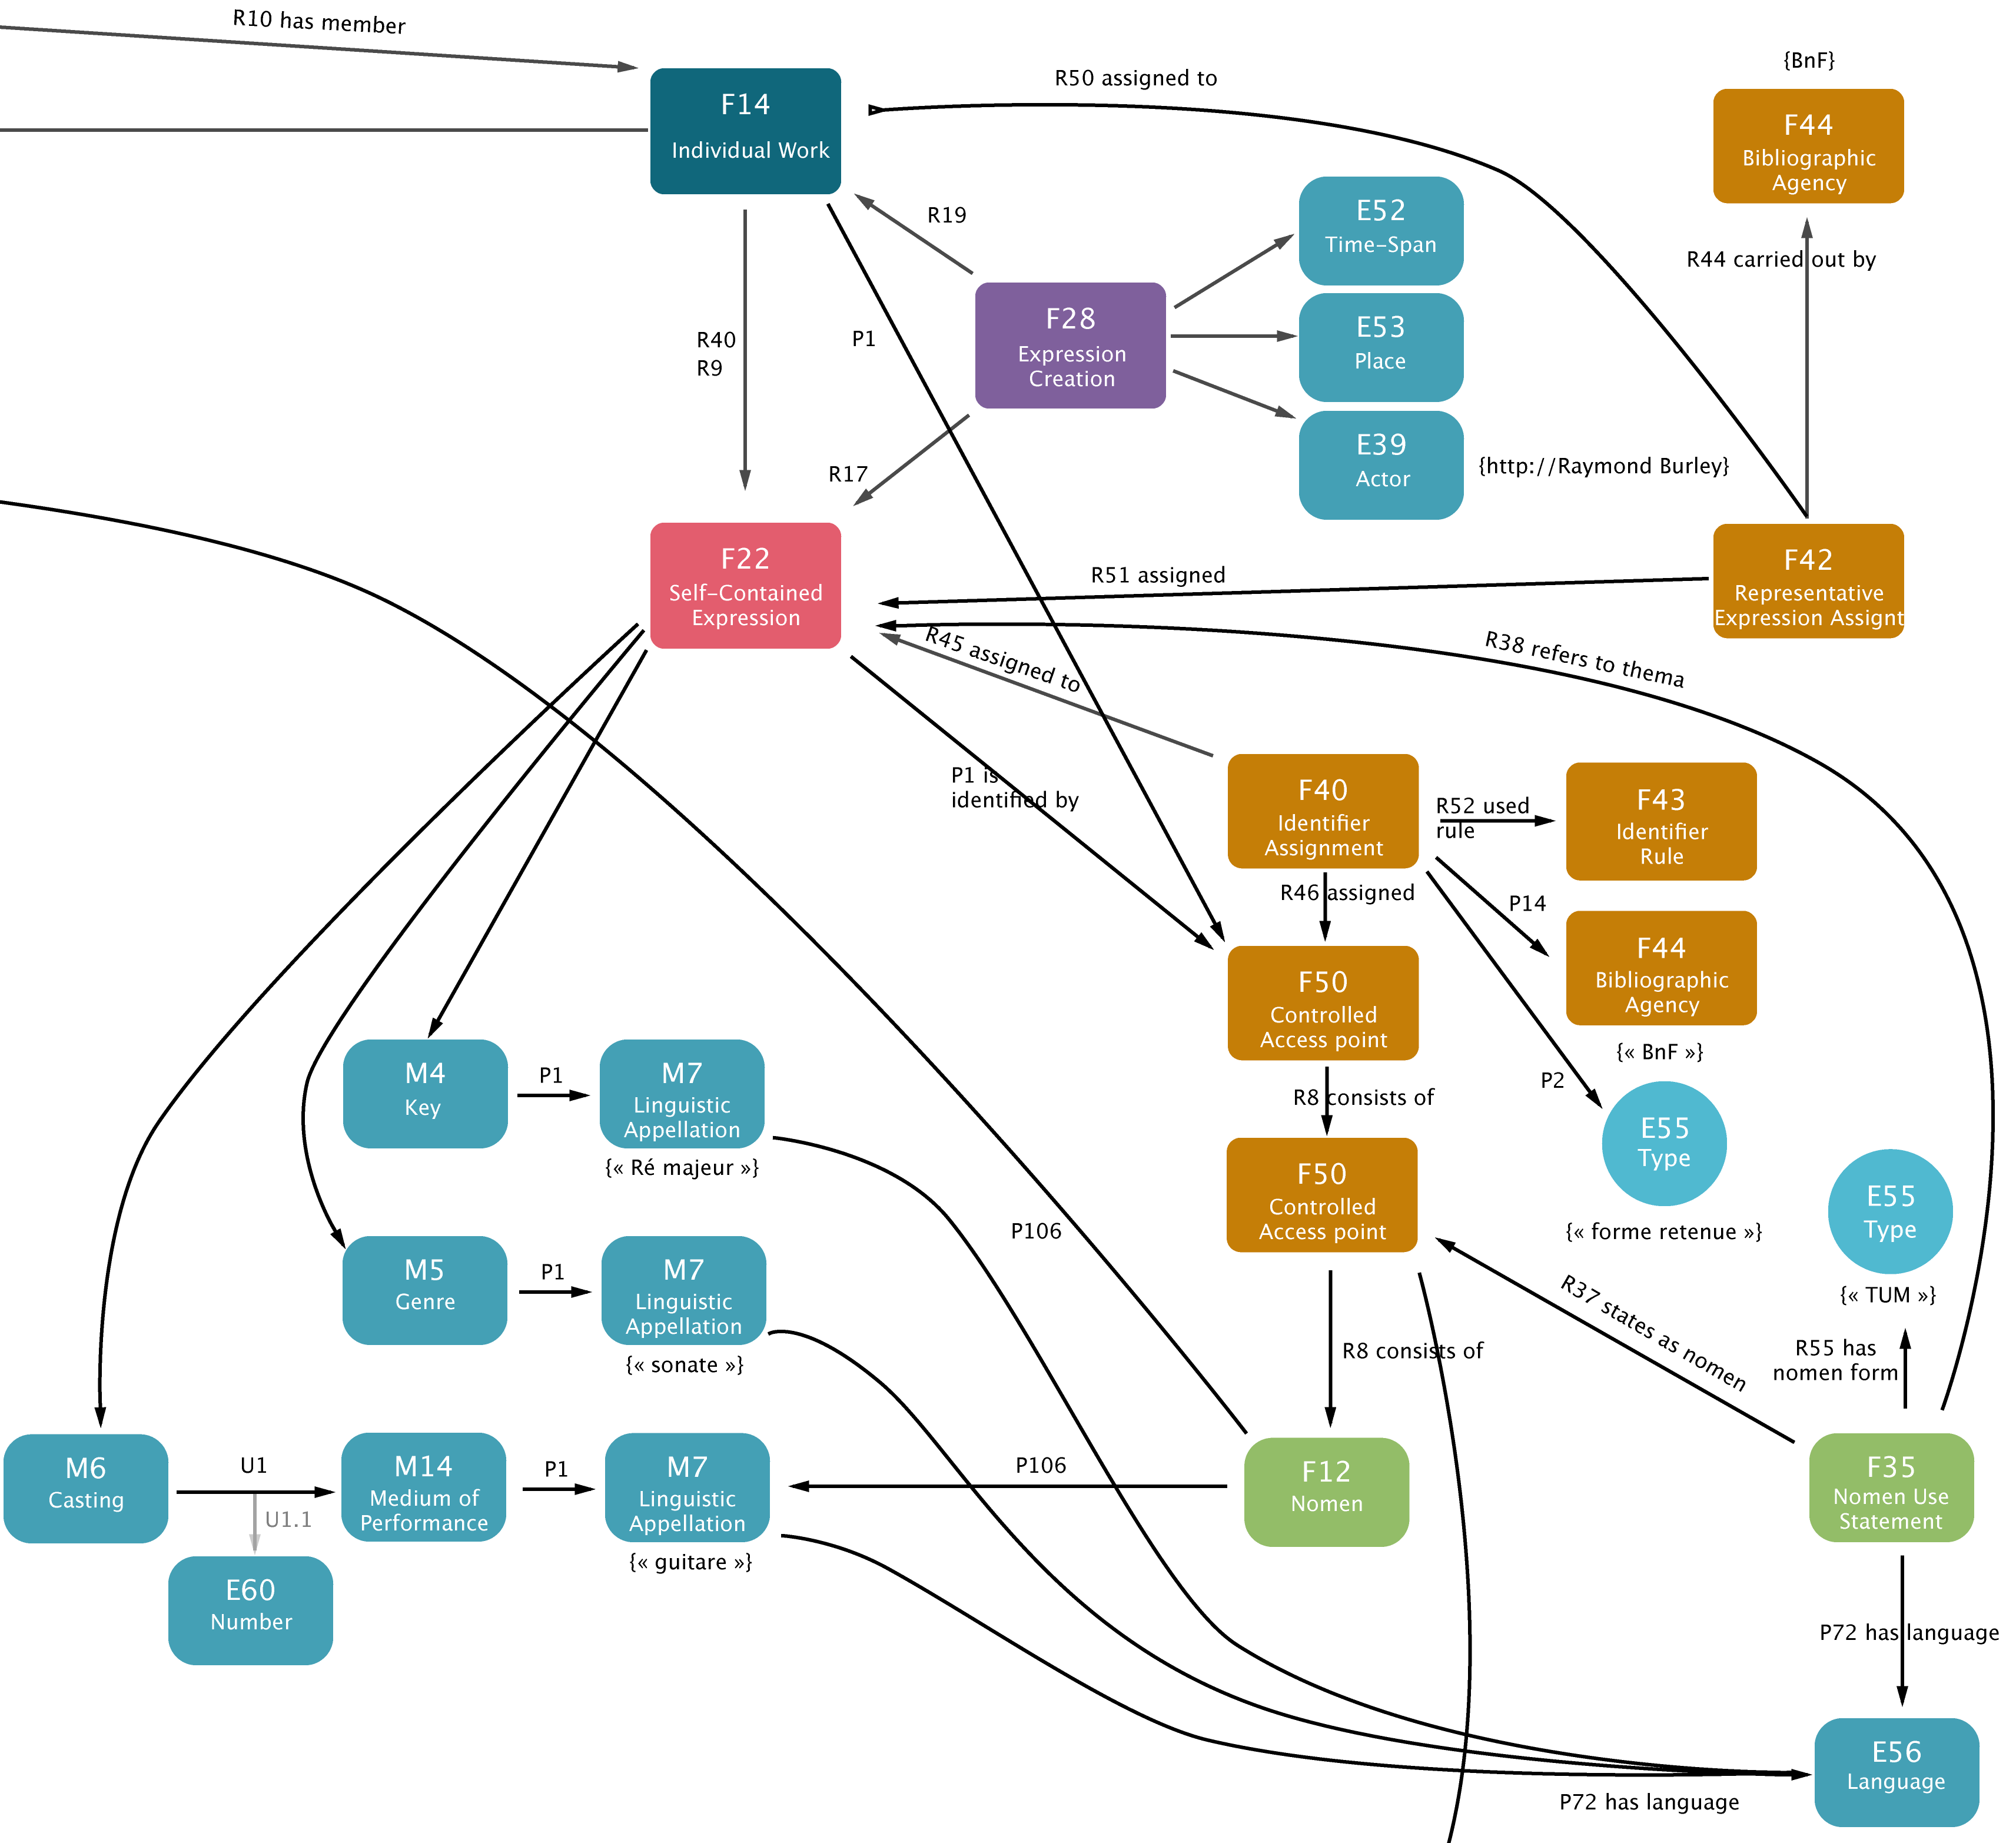
\includegraphics[height=6cm]{img/modelingdata_fig3.png}
  \caption{Modeling a musical work: M-classes and U-properties are extensions of FRBRoo}
  \label{fig:work}
\end{figure}

\vspace{-0.5cm}
One of the difficulties with musical works is that although their expressions may differ significantly, they are still regarded as a single work. Modeling it requires to express the singleness of the work as well as the specificities of its expressions, and to show how events are connected to these expressions. Another issue is that an arrangement may be considered as an expression or as a new work, depending on the data producer. Our model shall also make it possible to specify the relations between works, for instance when one work is derived from another.

We are currently working on a model enabling the expression of all these aspects in a coherent way, while being flexible and powerful enough to interoperate with information systems dealing with any kind of cultural data. It occurred to us that the FRBRoo ontology had all the required qualities. It is based on the FRBR and CIDOC-CRM  models, with a concern for the necessity to describe how events occur through the life of a thing and its resulting states. It is a formal ontology, based on the articulation of events and things, containing the notion of work, and offering precise elements to describe physical items. Its structure is adaptable and allows to model cultural metadata with fine granularity. Since the work, as defined in this model, is not specifically musical, we are extending the model by additional classes and properties that are recurrent and important in the description of musical works (Figure~\ref{fig:work}).

%%%%%%%%%%%%%%%%%%%%%%%%%
%%%  3. Data Lifting  %%%
%%%%%%%%%%%%%%%%%%%%%%%%%

\section{Data Lifting}
\label{sec:data-lifting}
As in many other domains, the DOREMUS project faces the problem of processing a very large amount of heterogeneous (in terms of formats and languages) and semi-structured data in order to transform them into RDF, describe them by (re-)using appropriate vocabularies, link these data to existing datasets and publish them on the web of data---a process also coined as \emph{data lifting}~\cite{scharffe2012enabling}. We have followed and adapted the workflow of the Datalift platform (Figure~\ref{fig:datalift}). The methods for extracting RDF triples need to be adapted to the data source in the musical field, which consists of documents in the MARC (MAchine-Readable Cataloging) format, as well as XML documents. %We also aim to address the challenges of multilingualism and data duplication since our three data providers have largely overlapping music catalogs.
\begin{figure}
  \centering
  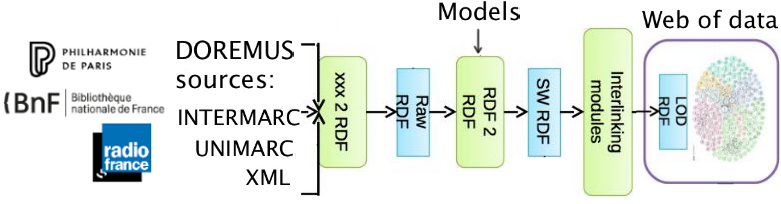
\includegraphics[width=10cm, height=1.5cm]{img/datalift-doremus.png}
  \caption{Data semantization and publishing workflow (adapted from~\cite{scharffe2012enabling}).}
  \label{fig:datalift}
\end{figure}

%\vspace{-0.5cm}
There exist several approaches for extracting RDF triples from XML documents~\cite{xml2rdf1}. However, MARC (and its variants) documents has, so far, been rarely processed by semantic web applications. We have developed a two steps approach for transforming MARC data into RDF, while dealing with two variants of the MARC format: UNIMARC and INTERMARC. First, we propose an approach to extract raw RDF at the highest possible level of granularity by exploiting subareas coded in MARC with an alphanumeric character and a delimiter $"\$"$ (Figure~\ref{fig:fig1}). The principle is that each area and sub-area will be represented by an RDF property and the RDF object has the value of the area or one of its subfields. Second, we perform a manual mapping between the UNI/INTER-MARC areas and sub-areas with classes and properties defined in the models discussed in Figure~\ref{fig:work}. Thus, the description of musical works is performed at a lower level of granularity (due to merging of certain subfields taken as values of a property), while ensuring completeness of the information.
\begin{figure}[htbp]
  \centering
  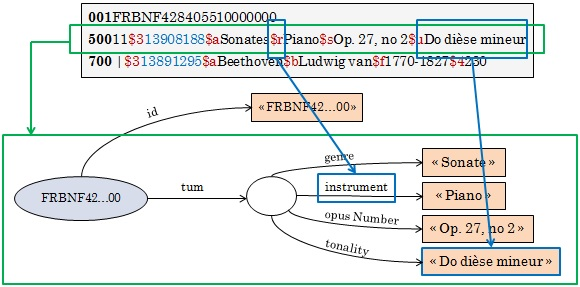
\includegraphics[width=10cm, height=3cm]{img/sonata.jpg}
  \caption{Transforming the UNIMARC version of the uniform musical title (TUM) of the {\it "Moonlight Sonata"} by {\it L.V.Beethoven} to RDF}
  \label{fig:fig1}
\end{figure}

Several documents within a single institution or across institutions describe the same entity (a particular musical work), but from different perspectives (scores, sound recordings, videos). We aim to develop generic data connectors~\cite{scharffe2012enabling} to automatically detect relationships (equivalence, transcription, interpretation) between musical entities. The multilingual nature of data---a characteristics that should be preserved in the data lifting process---will be handled by automating the alignment process of multilingual ontologies specific to the field of music.

%%%%%%%%%%%%%%%%%%%%%%%%%%%%%%%%%%%%%%%%%
%%%  4. Applications and Future Work  %%%
%%%%%%%%%%%%%%%%%%%%%%%%%%%%%%%%%%%%%%%%%

\section{Applications and Future Work}
\label{sec:applications}
Once the musical data coming from the cultural institutions is on the web of data, we plan to develop a musical recommendation application. It will serve as an evaluation of our model, and enable us to control the quality of data, after being modeled, lifted and interlinked. It will also be an example of how to implement the DOREMUS model for other cultural institutions.

The application will offer features such as the creation of original playlists for specialized radio, or the selection of appropriate musical works and interpretations to illustrate the biography of a composer, a historical period, culture or genre. The targeted end-users range from a child building his/her musical culture, through music lovers or curious discoverers, to expert musicologists.

%Once the musical data coming from the cultural institutions is on the web of data, we plan to develop several applications such as tools to support the recommendation of musical works for creating original playlists for specialized radio, or the selection of appropriate musical works and interpretations to illustrate the biography of a composer, a historical period, culture or genre. The targeted end-users range from a child building his/her musical culture, through music lovers or curious discoverers, to expert musicologists. Also, we plan to implement our proposal. In addition, we plan to conduct a large-scale extending and evaluation of our system to share musical data from various data sources. Finally, an interlinking recommandation tool based on musical data will be developped.

\section*{Acknowledgments}
This work has been partially supported by the French National Research Agency (ANR) within the DOREMUS Project, under grant number ANR-14-CE24-0020.

\bibliographystyle{abbrv}
\bibliography{bib-doremus}

\end{document} 